%*****************************************
\chapter{Future}\label{chapter:future}
%*****************************************

The primary focus of this thesis is a tractable implementation of a
cognitive architecture for the recursive application of reflective
layers of planning and learning.  Because the focus of this
dissertation has been on the larger recursive structure of the SALS
cognitive architecture, one layer of which is a closed-loop
non-reflective AI, each necessary sub-component of a single planning
layer in the SALS AI has been kept relatively simple.  Therefore, each
of these components of the current skeleton of the SALS AI can be
fleshed out in the future, while keeping the core tractable cognitive
architecture for a many-layered reflective AI.  The following are four
areas of research that would improve every layer in the SALS AI:
\begin{packed_enumerate}
\item{General partial state abstraction.  The ability to abstract more
  general partial states from a control domain would allow the
  addition of {\emph{critics}} that recognize relatively specific and
  intricate problematic partial states in the control domain, as is
  done in the EM-ONE architecture \cite[]{singh:2005b}, the precedent
  for this work.}
\item{A propagation model of knowledge maintenance that traces
  knowledge provenance from refined hypotheses learned from experience
  to plan goal accomplishment and avoidance hypotheses
  \cite[]{radul:2009}.  Currently, the SALS AI must completely
  re-imagine the effects of a plan when new hypotheses are learned
  from experience.}
%% \item{Currently, the SALS AI is limited to the same simple conjunctive
%%   hypothesis space for each reflective layer.  Learning of hypothesis
%%   priors that predict which hypothesis spaces may contain the correct
%%   hypothesis for specific types of resource executions and problem
%%   domains.  In Bayesian terms, a general approach could amount to
%%   learning hierarchical hypotheses over structured priors
%%   \cite[]{mansinghka:2012}, adapted in order to learn a distinct
%%   hierarchical model of priors for each reflective planning layer
%%   domain in the SALS AI.}
\item{General grammar definitions in the natural language programming
  language, such as those presented by \cite{winograd:1970}.
  Currently, the SALS natural programming language is limited to a
  simple functional grammar.}
\item{More efficient usage of multicore, hyperthreaded, and
  multiple-processor hardware platforms as well as completion of the
  distributed processing model that is partially implemented in the
  memory layer of the SALS virtual machine, which would allow
  peer-to-peer distributed processor support.}
\end{packed_enumerate}
In addition to making improvements to the existent structure of the
SALS AI, there are a number of aspects missing from the SALS AI that
could be added to the architecture in order to better model human
commonsense thinking.  A few selected ideas for new additions to the
SALS AI are as follows:
\begin{packed_enumerate}
\item{Self-reflective and self-consciously reflective thinking, the
  top two layers of the Emotion Machine theory of human commonsense
  thinking \cite[]{minsky:2006}, including self-models and social
  knowledge.}
\item{Extending reflective planning layers downward into the domain of
  plans-to-perceive \cite[]{pryor:1992,pryorcollins:1995,velez:2011},
  so that the SALS AI can learn plans for abstracting spatial
  relations between symbolic perceptions, such as the visual routines
  first implemented by \cite{ullman:1984}.}
\item{Plan and meta-plan recognition as a way to include current
  research on reflective story understanding architectures that
  attempt to explain the actions of actors in terms of goals and
  meta-goals that the actor may be trying to accomplish
  \cite[]{wilensky:1981,cox:1999b,cox:2010,winston:2011}.}
\end{packed_enumerate}

\section{General Partial State Abstraction}

The SALS AI is currently restricted in the types of partial states
that it can abstract from the knowledge base that it is trying to
control.  The two types of partial states that are included in the
current implementation are the ``{\tt{relationship}}'' and
``{\tt{property}}'' types that have been described in
{\mbox{\autoref{chapter:learning_from_being_told}}}.  Implementing
more general types of partial state abstraction in the SALS AI must be
done carefully in order to keep the architecture tractable at higher
layers.  One goal for implementing perceptual partial state
abstractions of greater complexity would be to allow for implementing
critics from EM-ONE \cite[]{singh:2005b}.  Putting efficiency aside
for the moment, implementing new types of partial state abstractions
for the SALS AI is a straightforward task.  There are two places in
each planning layer where partial state abstraction processes are
executed:
\begin{packed_enumerate}
\item{\emph{Asynchronous Procedural Event Stream Abstraction}: The
  asynchronous learning algorithm that exists in each reflective layer
  abstracts partial states from a historical reconstructed copy of the
  knowledge base that the planning layer is trying to control.}
\item{\emph{Direct Real-Time Read Abstraction}: An executing plan may
  execute a procedure that checks to see if a specific type of partial
  state currently exists in the knowledge base that it is trying to
  control.}
\end{packed_enumerate}
Asynchronous learning from procedural event streams requires that when
a planning layer receives a change event from the knowledge base in
the layer below, the planning layer integrates this change into a
reconstructed copy of that knowledge base.  The reconstructed
knowledge base represents the state of the knowledge base that the
planning layer is trying to control at a point in the past.  The
asynchronous abstraction process works on this reconstruction in order
to determine whether or not the change has either created a new
instance of a type of partial state or has removed a previously
existing instance.  The asynchronous procedural event stream
abstraction of partial state types works in order to learn causal
hypotheses for the effects of resource executions in the layer below.
When a plan is currently executing in the planning layer, it is
sometimes useful to determine whether or not a specific partial state
currently exists in the knowledge base that the planning layer is
trying to control.  The asynchronous partial state abstraction cannot
be used for this type of real-time query because the asynchronous
abstraction algorithm works on an historical copy of the knowledge in
question.  Therefore, the direct real-time read abstraction of a
specific partial state from the current state of the knowledge base is
sometimes necessary for this purpose.

In order to demonstrate the difference in time-complexity between
these two methods of abstracting types of partial states, let us
consider that a partial state is a specific subgraph that is to be
symbolically reified both asynchronously as well as by direct read
access from a graph representation of the frame-based knowledge base
that the planning layer is trying to control.
{\mbox{\autoref{figure:general_partial_state_arch}}} shows an example
of a more complex type of partial state than the SALS AI can currently
abstract, which represents an ``arch,'' similar to the arch category
learned by near-miss learning by \cite{winston:1970}.
\begin{figure}
\centering
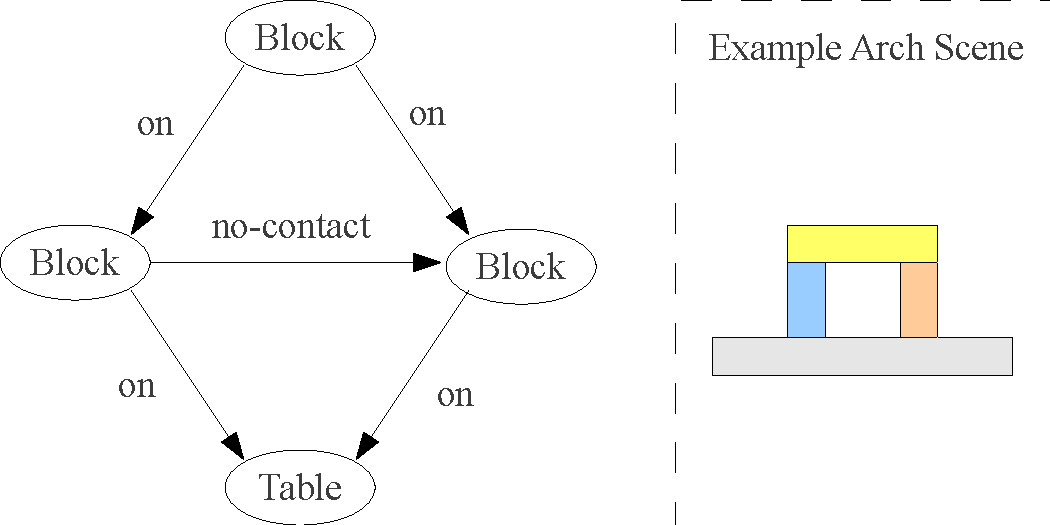
\includegraphics[width=10cm]{gfx/general_partial_state_arch}
\caption[An example of a more complex type of partial state than the
  SALS AI can currently abstract, which represents an arch.]{An
  example of a more complex type of partial state than the SALS AI can
  currently abstract, which represents an arch.}
\label{figure:general_partial_state_arch}
\end{figure}
As these types of partial states become more complex, the direct
real-time read approach to abstraction becomes very similar to the
NP-complete subgraph isomorphism decision problem, which quickly
becomes intractable for large subgraphs.\footnote{Given a set of
  subgraphs that are of interest, preprocessing these subgraphs can
  lead to a practically more efficient hierarchical ``graph
  stitching'' algorithm for finding which of this set of subgraphs
  exist within a target graph \cite[]{messmer:1995,messmer:2000}.  For
  large enough graphs, however, these algorithms are still intractable
  for real-time queries.  These algorithms have been implemented and
  are included in the SALS AI, but are not used for the examples in
  this dissertation.}

Consider how the asynchronous abstraction of subgraphs from change
event streams can improve upon the intractable subgraph isomorphism
problem.  The key to realize is that the change event focuses the task
of the asynchronous abstraction process, which changes the general
graph isomorphism problem into a focused tree matching problem, given
that spanning trees are precomputed for each edge in the partial state
graph of interest.
{\mbox{\autoref{figure:general_partial_state_arch_spanning_trees}}}
shows an example of five minimum spanning trees, one for each edge of
the arch example partial state.  Computing a minimum spanning tree for
a connected graph has polynomial (FP) time-complexity.  Precomputing
one minimum spanning tree rooted at each edge in the partial state of
interest reduces the general NP-complete graph isomorphism decision
problem to a rooted tree matching problem.
\begin{figure}
\centering
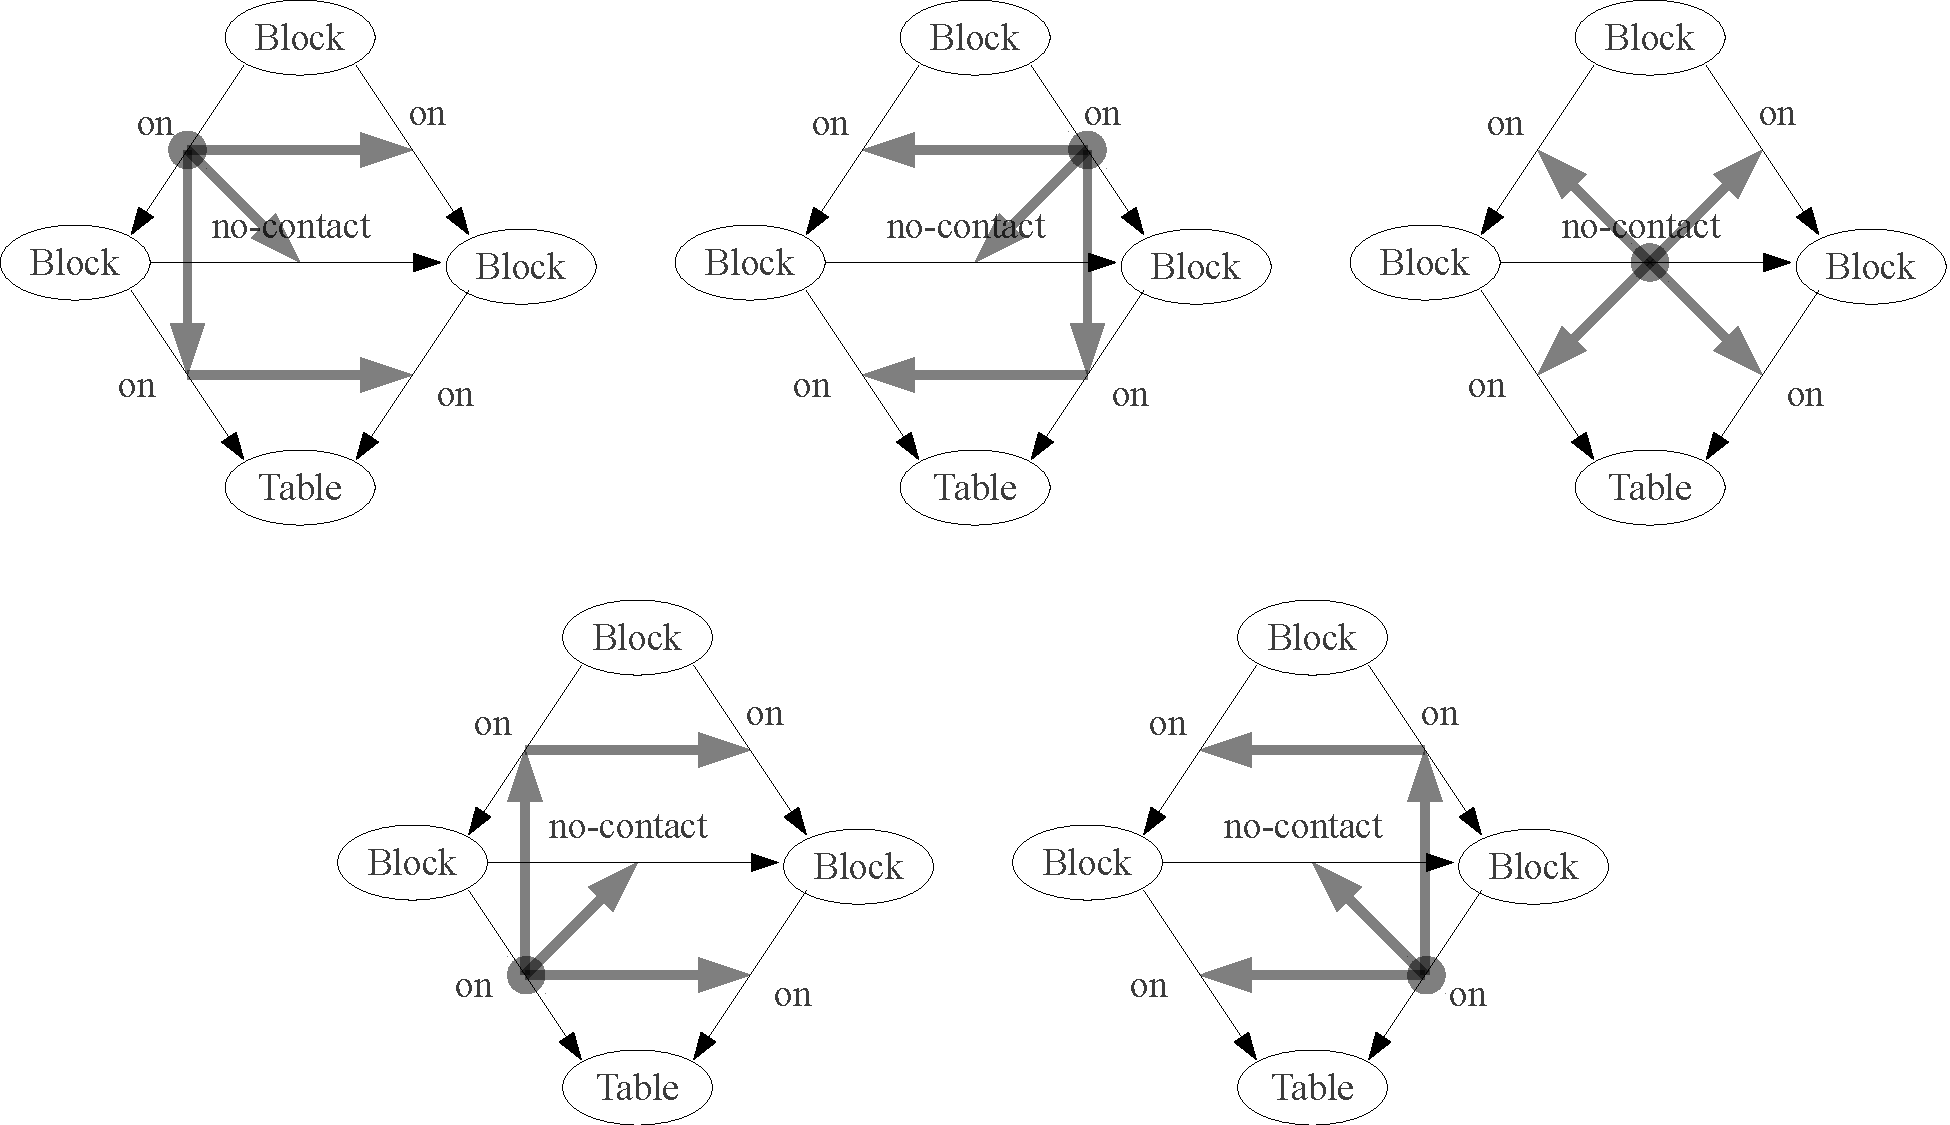
\includegraphics[width=12cm]{gfx/general_partial_state_arch_spanning_trees}
\caption[Five minimum spanning trees between the edges of the arch
  example partial state.]{Five minimum spanning trees between the
  edges of the arch example partial state.  One minimum spanning tree
  is shown for each edge in the partial state of interest.
  Precomputing one minimum spanning tree rooted at each edge in the
  partial state of interest reduces the general NP-complete graph
  isomorphism decision problem to a rooted tree matching problem.}
\label{figure:general_partial_state_arch_spanning_trees}
\end{figure}

While there may be a more efficient solution to the asynchronous
abstraction of partial states in the SALS AI, the problem of real-time
abstraction is still an NP-complete problem.  I do not see any easy
solutions to this problem, but there are two ways that I see to avoid
it.  One way to avoid the problem is to limit the real-time partial
state abstraction to a predefined set of small graphs that only
involve 5 to 10 nodes.  \cite{messmer:1995} describes an efficient
algorithm for this type of query.  Note that this type of query would
still allow the asynchronous learning of causal models from partial
states with precomputed minimum spanning trees rooted at change
events.  Another way to avoid the NP-complete problem of real-time
abstraction of partial states is to ignore it.  If the asynchronous
abstraction of partial states can run quickly enough, perhaps by
allocating a parallel processor and a separate reconstructed knowledge
base to each type of partial state, the asynchronous algorithm could
potentially show little enough latency to make it near enough to
real-time to be practically useful.

\section{Propagation by Provenance of Hypothetical Knowledge}

Currently in the SALS AI, when a resource is executed by a planning
layer, generalized hypotheses are learned that are used to predict the
effects of those resource executions in the future.  For example,
these hypotheses are used to predict the effects of a plan when that
plan is imagined being executed as part of the planning process in a
planning layer.  When a plan is imagined in this way, these effects
are associated with the plan object in the plan knowledge base of that
layer.  Subsequently, when the hypotheses that support these
conclusions are refined due to new experience gained through the
execution of similar plans or actions, the hypothetical support for
these original conclusions may be lost.  The problem is that these
original conclusions remain associated with the plan objects, even in
the case when the hypothetical support for those conclusions is lost
through the refinement of the hypothesis spaces from which they were
originally derived.  Because of the potential loss of hypothetical
support for the effects of plans, the plan must be completely
re-imagined whenever the asynchronous learning algorithms have learned
new information through the experiential event streams.

\cite{radul:2009} explain a type of Truth Maintenance System (TMS)
\cite[]{doyle:1978} called a {\emph{propagator}}.  A propagator
network is composed of {\emph{cells}} that represent variables in a
computational process that can have multiple ambiguous values.  The
propagator network also has the ability to track the provenance of the
derivations for the values stored in these cells.  The advantage of
TMSs and propagator networks is the ability to perform dependency
directed backtracking in order to find new justifications for beliefs
when contradictions in knowledge are encountered.  If the knowledge
derivations in the SALS AI were built based upon a propagator network,
the contradictions between hypothetical assumptions and new
experiential input could be propagated efficiently to the effects that
are associated with plan objects.  One advantage of propagator
networks over traditional TMS systems is their ability to maintain
multiple possibly contradictory sets of beliefs that are derived from
different sources of information.  The ability to maintain multiple,
possibly conflicting belief structures in a propagator network would
allow the SALS AI to consider the source of the knowledge and develop
ways of reasoning that determine when one source is more reliable than
another.  For example, when the SALS AI learns new plans from being
told, the source of this knowledge could be associated with different
users or other specific AIs that are the source of these new
assertions.  When one source is found to be valid for one domain but
invalid for another, the SALS AI could use the features of a
propagator network to easily switch between reasoning using different
sets of knowledge sources in different circumstances.

%% \section{Learning Hypothesis Space Priors}

%% Currently, the SALS AI is limited to the same simple conjunctive
%% hypothesis space for each reflective layer.  Learning of hypothesis
%% priors that predict which hypothesis spaces may contain the correct
%% hypothesis for specific types of resource executions and problem
%% domains would be a useful addition to the SALS AI.  In Bayesian terms,
%% a general approach could amount to learning hierarchical hypotheses
%% over structured priors \cite[]{mansinghka:2012}, adapted in order to
%% learn a distinct hierarchical model of priors for each reflective
%% planning layer domain in the SALS AI.

\section{General Natural Language Grammar}

The SALS AI currently interprets natural language plans, while
simultaneously considering syntax, semantics, current environmental
context, learned hypothetical knowledge about the effects of actions
as well as the current positive and negative goals of the AI.  The
SALS natural programming language is currently limited to a simple
functional grammar.  One problem with many natural language grammars
are that they usually assume a specific language, such as English, as
the basis for their grammar.  Although the SALS AI grammar is simple,
the benefit of this simplicity is that because it is based on a
Unicode string matching template, it is able to represent and reason
with natural language phrases from any natural human language,
including languages like Chinese and Japanese, which do not have words
separated by spaces.  While there are many ways to improve the SALS
natural language interpreter, the following are four that are
immediately applicable to the SALS AI:
\begin{packed_enumerate}
\item{\emph{Mutation, Side-Effects and Causal Variables}: One
  immediate way to maintain the generality of the SALS natural
  language interpreter, while adding the complexities of a general
  natural language grammar, is to allow the language to have mutation
  side-effects, so that the interpreter can be stateful.  Adding
  mutation side-effects to the SALS natural language interpreter
  introduces a complexity to the current interpretation search process
  that would become intractable without an explicit additional method
  of curbing this complexity.  Dependency tracing would be a promising
  way to reign in the complexity of this search process.}
\item{\emph{One Consolidated Natural Language Interface}: The SALS AI
  currently receives natural language plans through a separate
  interface to each planning layer.  One future goal for the
  architecture is to have one natural language input to the entire
  architecture that enters the architecture through the lowest-level
  perceptual knowledge bases of the built-in reactive layer and
  propagates upward through the planning layers until the natural
  language phrase is completely understood.}
\item{\emph{Incremental Natural Language Understanding}: In order to
  increase the realism of the SALS natural language interpreter, the
  ability of the interpreter to receive and process a stream of
  phonetic or character-level symbols in temporal order, rather than
  in template form, could allow the SALS AI to begin imagining
  multiple possible interpretations of a statement or phrase before
  that statement or phrase has been completely communicated to the
  SALS AI.}
\item{\emph{Natural Language Analogies Between Layers}: The inherent
  ambiguity of natural language plans allows analogies to be made
  between plans within any given planning layer.  An exciting avenue
  for future research is the creation of analogies between planning
  layers in the SALS AI.  For example, consider that the AI has
  learned a plan for stacking blocks in the Blocks World domain that
  involves first dividing the blocks into two groups on the table: (1)
  cubes and (2) pyramids.  The AI can execute a simple block stacking
  plan that simply selects blocks from the group with only cubes in
  order to create a stack without again considering the shapes of the
  blocks in question.  This plan for physical action, could provide an
  analogy for the reflective thinking layer if the AI confronts a
  problem that requires plans to be grouped into two lists: (1) those
  plans that activate resources concurrently, and (2) those plans that
  execute resources sequentially.  This could be a way to plan quickly
  without imagining potential resource conflicts in plans with
  concurrent resource executions.  Finding analogies between natural
  language plans of different layers in the SALS AI could lead to
  faster learning in new domains of reflective thinking, for example,
  if the AI knew many plans for physical action and few for reflective
  action.}
\end{packed_enumerate}
Natural language plans are an important part of a cognitive
architecture because of the potential for the AI to be able to explain
its own reasoning processes in terms of this natural language
understanding.  There are many directions for extending the use of
natural language in the SALS AI.

%% \section{Distributed Hardware Support}

\section{Self-Reflective Thinking}

The {\emph{self-reflective}} and {\emph{self-conscious}} layers are
the top two layers of the Emotion Machine theory of human commonsense
thinking \cite[]{minsky:2006}.  These two layers are not included in
the current version of the SALS AI.  The self-reflective layer
includes plans that control the planning resources in the lower
reflective layers.  The self-reflective layer contains
{\emph{self-models}} which represent large-scale reconfigurations of
the thinking resources in the lower reflective layers of the AI.
These global changes to the way an AI is thinking are sometimes
referred to as ``emotions'' or ``personalities'' depending on the
time-scale.  My usage of these terms is analogous to the usage of the
terms ``weather'' and ``climate.''  A personality is a longer-term
plan involving shorter-term emotion actions.  The following is a list
of some simple emotion and personality plan definitions that could be
added to a self-reflective layer of the SALS AI:

\begin{packed_itemize}
\item{Be happy: Do nothing.}
\item{Be tired: Make a plan to go to sleep.}
\item{Sleep: Imagine executing recently used plans in a variety of
  contexts.}
\item{Be frustrated: Try to find goals to give up that are not worth
  accomplishing.}
\item{Grieve: Replace old plans and goals that depend upon lost
  resources.}
\item{Be athletic: Get better at making plans that require me to exercise.}
\item{Be friendly: Get better at making plans to help friends accomplish their goals.}
\end{packed_itemize}

\noindent The self-reflective layer's plan knowledge base could include the
following types of self-model knowledge, which would be reflections of
the above plans being executed:

\begin{packed_itemize}
\item{I am happy.}
\item{I am tired.}
\item{I am frustrated.}
\item{I am grieving.}
\item{I am athletic.}
\item{I am friendly.}
\end{packed_itemize}

\noindent One distinguishing factor of the self-reflective layer is
that it not only includes self-models but also analogous
{\emph{other-models}}.  The following is a list of other-model
knowledge:

\begin{packed_itemize}
\item{Joe is happy.}
\item{Carol is tired.}
\item{Carol is frustrated.}
\item{Suzy is grieving.}
\item{Ralph is athletic.}
\item{Lauren is friendly.}
\end{packed_itemize}

\noindent The self-reflective layer has the capability to abstractly
simulate self-models and other-models in terms of all of the partial
states in the layers below.  This simulation can probably be performed
tractably because only a linear increase in complexity has been seen
to be added to the SALS overall architecture with each additional
layer in the current architecture.

One way to simulate other-models and self-models analogously is by
adding an ontology to the SALS AI's knowledge bases.  Currently the
SALS AI can only abstract and simulate symbolically reified partial
states that represent the problem domain.  These collections of
symbols that are the input to each planning layer of the SALS AI are
not {\emph{object-oriented}}.  Meaning that they are not organized
into frame-based object representations.  Learning an ontology of
object types is future research for the SALS AI.  The ability to
abstract and simulate object types may be related to learning object
binding affordances \cite[]{stoytchev:2005}.  Also, learning these
object types may lead to an object model that could naturally be
extended for learning self-models and other-models.

\section{Self-Conscious Thinking}

The {\emph{self-conscious}} layer is the top layer of the Emotion
Machine theory of human commonsense thinking.  The self-conscious
layer is a planning layer that controls the self-reflective layer
below.  Self-conscious thinking involves thinking about what one
person is thinking about another person.  The representations in the
self-conscious thinking layer include relationships between
self-models and other-models from the self-reflective layer.  The
following are examples of self-conscious knowledge:
\begin{packed_itemize}
\item{Joe is imagining that Lauren is happy.}
\item{Ralph is unaware that Suzy is grieving.}
\item{Carol imagines that Ralph knows a plan to stack two blocks.}
\item{Lauren knows that I failed to stack two blocks.}
\item{Ralph and Lauren are Suzy's children.}
\end{packed_itemize}
The self-conscious thinking layer is the first reflective layer in the
Emotion Machine theory to include reasoning about the roles of
individuals in the context of social groups.  \cite{minsky:2006}
explains one of these types of relationships that allows the direct
inheritance of high-level goals from one agent to another agent that
he calls the {\emph{imprimer}} relationship.  An imprimer functions in
a developmental situation where a learner inherits high-level goals
from their imprimer.  A parent or caregiver in the context of raising
a child might be seen as imprimers to the developing child that teach
the child what kinds of social roles, personality traits, and other
ways of thinking should be practiced or ignored.

\section{Planning to Perceive}

{\mbox{Section~\ref{section:meta_planning_and_meta_plan_recognition}}}
describes the {\emph{Architecture for Visual Routines (AVR)}}
\cite[]{rao:1998} that is based on an idea originally proposed by
\cite{ullman:1984}.  To briefly review, {\emph{visual routines}}
define objects and parts by having a visual plan interpreter that is
focused on a specific part of the low-level visual input at any given
point in time.  Although the first planning layer in the SALS AI is
the deliberative layer, one can imagine that a solution to including a
perceptual planning layer would be to extend the SALS planning layers
into the learned reactive layer of the SALS AI, so that the
translation of visual knowledge from the built-in reactive visual
knowledge base to the physical knowledge base in the learned reactive
layer would be performed by a planning layer below the deliberative
layer.  Thus, the technique of extending the SALS AI's planning layers
to higher layers of super-reflective control could be just as easily
reversed by extending the SALS AI's planning layers to lower layers of
planned control, so that reflective control could be applied to the
types of planning-to-perceive problems as a coherent integration of
Ullman's visual routines into deliberative reasoning layers of
reflective control.

\section{Plan Recognition and Story Understanding}

{\mbox{\autoref{section:meta_planning_and_meta_plan_recognition}}} has
described the relationship between the planning implemented in the
SALS AI and the related problems of plan recognition, meta-plan
recognition, and story understanding.  To briefly review,
\cite{wilensky:1981} describes story understanding as a form of
inverse planning or plan recognition.  In this sense, a planning
system is given a set of goals that are used to generate a sequence of
actions that accomplish the goals, while a story understanding system
is given a sequence of actions that are used to generate a set of
goals that explain those actions.  Wilensky emphasizes that both story
understanding and planning require representations of meta-goals and
meta-plans in order to reason about common types of human thinking.
Plan recognition could occur analogously in each layer of the SALS AI.
Resource executions are the actions of each planning layer.  The plan
recognition problem for the deliberative layer could be considered to
be a problem that takes a collection of resource execution events and
gives as output the goals that these actions could be hypothetically
trying to accomplish.  One method for accomplishing this would be to
compare the input traces to the imaginative traces from executing each
plan for physical action, then, hypothesize the goals that the plans
with matching traces are hypothesized to cause.  Currently, the SALS
AI is directed more toward planning, so that plans for plan
recognition can be reflected upon by the SALS AI.  The SALS AI is
currently more of a planning system than a plan recognition system for
one simple reason: methods for plan recognition can be written in the
planning system so that they can be automatically learned about and
debugged by the SALS AI.

%% \section{from related models (EM-ONE)}

%% The EM-ONE architecture does not have an explicit self-reflective
%% layer that contains these types of self-reflective thinking.  The SALS
%% AI makes an attempt to keep a clear distinction between the types of
%% knowledge that are available to each reflective layer of mind.  The
%% SALS AI does not contain self-reflective knowledge in its deliberative
%% or reflective layers of thinking because if this knowledge is allowed
%% to exist in these lower layers, this introduces ``loopy'' knowledge
%% references that confuse the purely hierarchical control structure that
%% currently exists in the SALS AI.  For example, the deliberative layer
%% of the SALS AI can only manipulate physical knowledge as the
%% reflective layer in the SALS AI can only reference deliberative
%% knowledge and indirectly reference the physical knowledge that the
%% deliberative knowledge references.  The fact that the reflective layer
%% in the SALS AI cannot reference higher layers of reflective knowledge,
%% such as self-reflective knowledge, is consistent with the SALS
%% architecture's strictly hierarchical knowledge organization between
%% reflective layers of control.  The SALS AI is currently limited to the
%% knowledge of the bottom four layers of the Emotion Machine
%% architecture.

%% \section{from related models (metacognition)}

%% The Emotion Machine theory makes a distinction between layers of
%% reflective knowledge and self-reflective knowledge that is not clearly
%% distinguished in the metacognitive theory.  The implemented SALS
%% architecture is currently only an implementation of reflective
%% thinking but implementing self-reflective thinking, what the cognitive
%% science literature would refer to as ``theory of mind,'' will be
%% described as a future extension of the SALS architecture in
%% {\mbox{\autoref{chapter:future}}}.  The Emotion Machine theory of
%% self-reflective thinking is a higher-level form of thinking than
%% simply reflecting and controlling a deliberative or object level
%% thought process.  The Emotion Machine theory of self-reflective
%% thinking describes how humans think of themselves and others in terms
%% of abstract models of their ``selves,'' different subpersonalities
%% that depend on the current problem solving or social context.
%% \cite{minsky:2006} begins his description of ``selves'' as analogous
%% to how one might think of others:
%% \begin{quote}
%% How do people construct their Self-models?  We'll start by asking
%% simpler questions about how we describe our acquaintances.  Thus, when
%% Charles tries to think about his friend Joan, he might begin by
%% describing some of her characteristics.  These could include his ideas
%% about: the appearance of Joan's body and face, the range and qualities
%% of her abilities, her motives, goals, aversions, and tastes, the ways
%% in which she is disposed to behave, her various roles in the social
%% world.
%% \end{quote}
%% {\mbox{\autoref{figure:emotion_machine_multiple_models_of_self}}}
%% shows a few examples of different subpersonalities or ``selves'' that
%% Minsky explains a person may use to think in different contexts.
%% \begin{figure}
%% \centering
%% \includegraphics[width=8cm]{gfx/emotion_machine_multiple_models_of_self}
%% \caption{Multiple models of self.}
%% \label{figure:emotion_machine_multiple_models_of_self}
%% \end{figure}
%% The metacognitive meta-level could be said to map to both reflective
%% and self-reflective layers of thinking in the Emotion Machine.


%% \section{old beginning}


%% The Emotion Machine cognitive architecture has interesting
%% implications for the future of AI.  The ability to reflectively learn
%% in $n$ layers has not yet been shown, but the linear slowdown of this
%% implementation with the addition of reflection, along with the
%% potential for no slowdown on ideal concurrent shared memory
%% architectures point toward learning much more useful information in
%% one-shot learning situations, where learning is costly or dangerous.

%% \section{Learning Object and Subject Distinctions}
%% \label{section:objective_reflection}

%% Although this model is based upon an assumption of objects and their
%% relationships, the ability of the AI to learn new object type
%% abstractions and subjective perspectives is future research for the
%% architecture.  Having the architecture abstract its own types of
%% objects and ways of using these objects would be useful in the
%% deliberative layer for learning physical object types, but the ability
%% to abstract object types and subjective perspectives becomes more
%% interesting in the metacognitive layers because this may lead to
%% concepts of problems as types of objects that may be solved through
%% different representational perspectives.

%% The ability to abstract object and subject distinctions within the
%% mind is a key that may lead to the abstraction of a concept of
%% ``self'' objects within the AI, as it makes distinctions between those
%% physical objects that it thinks of as its body versus those physical
%% objects that it thinks about as an environment.  The most important
%% and the first subject and object distinctions may be those that help
%% accomplish or avoid physical goals.  The separation between the
%% physical body and the physical world is an objective form of thinking
%% that could partially be caused by goals that emphasize distinguishing
%% bodily and worldly goals in the causal structures of the physical type
%% knowledge.  For example, \cite{bongard:2006} demonstrates an approach
%% referred to as ``motor babbling'' that uses a non-reflective model in
%% order to learn a physical self-model.

%% \section{The Self-Conscious Layer and Social Goals}

%% If we are going to develop a theory of social goals, how do we begin
%% to model the cooperative and non-cooperative thought processes that
%% would constitute working toward or against other people? It has been
%% shown that the neural circuits that are involved in how someone thinks
%% about what someone else knows are largely distinct from the circuits
%% involved in perceptual capabilities \cite[]{bedny:2009}. There have
%% also been distinctions shown between the neural circuits involved in
%% how someone thinks about what someone else knows and executive control
%% of actions \cite[]{saxe:2006}. There is good reason to believe that
%% the learning of social behavior is bootstrapped from learning causal
%% physical models \cite[]{perner:1991}.

%% \section{A Physically Grounded Social Problem Domain}

%% The IsisWorld simulation \cite[]{smith:2010} is a rigid-body physics
%% simulation that is capable of handling semantic commonsense objects
%% and actions involved in kitchen cooking tasks.  In order to help us
%% define a grounded problem domain, I have chosen to focus on a
%% rigid-body physical simulation of parents and children in the context
%% of basic cooking tasks in a kitchen environment. I chose parents and
%% children because I feel that major parts of social learning develops
%% during early stages involving these familiar social relationships. I
%% chose the domain of basic kitchen cooking tasks because this is a
%% non-trivial social commonsense reasoning domain that exists in some
%% form in all human cultures.

%% \section{The Self/Other Distinction and Self-Reflective Thinking}

%% I have described \cite[]{morgan:2011} a theory of how self-reflective
%% states are communicated or inferred in other agents by correlating a
%% physical perceptual stream with a reflective perceptual stream,
%% allowing the agent to use these correlations to predict the reflective
%% states of other agents based purely on their physical actions. For
%% example, if one agent performs a series of physical actions in order
%% to accomplish a goal, such as preparing a slice of buttered toast
%% using a knife and a loaf of bread and some butter in a kitchen, then
%% these actions have been correlated with this agent's reflective
%% states, including the current goals that the agent is pursuing. If
%% this agent then sees the physical world changing, and he knows that he
%% is not causing those changes, then he can attempt to infer the state
%% of mind of another agent. This type of inference process, based on the
%% previous correlations of physical and reflective perceptual streams,
%% is what could be referred to as a self-reflective thought process. A
%% self-reflective thought process introduces the social distinction
%% between Self and Other reflective state knowledge that is inferred by
%% using the previously learned correlations between physical perceptions
%% and reflective perceptions.  This is a type of self-reflective
%% knowledge that is knowledge that allows thinking about what someone
%% else is thinking about.  Sometimes this self-reflective knowledge is
%% referred to as "theory of mind" knowledge in the cognitive science
%% literature.

%% With self-reflective knowlege, an agent can choose to act
%% altruistically by helping another agent accomplish their goals or
%% maliciously by working against their goals. However, there is the
%% possibility that an agent is not always running a self-reflective
%% process that pays attention to another agent's physical actions in
%% order to infer what their goals might be. In many cases, such as in
%% the IsisWorld physical simulation of parents and children in a
%% kitchen, some agents might focus single-mindedly on a novel task
%% without thinking about what the goals of surrounding agents might
%% be. This type of model allows for an agent that works against the
%% goals of another agent without knowing the goals of the other
%% agent. One might argue that this type of situation where one agent
%% clobbers the goals of another agent is due to a form of
%% self-reflective laziness and not due to malicious intentions.

%% \section{Guilt, Pride, and Self-Conscious Thinking}

%% It is interesting to consider how children learn from parents as well
%% as how parents guide a child's cooperative behavior, but to study this
%% type of thinking, the AI must be extended in order to allow for
%% modeling what one agent thinks about what another agent thinks about
%% her.  This form of double reflective recursion is self-conscious
%% knowledge and the problems that are represented in this type of
%% knowledge are handled by what is called self-conscious thought
%% processes. For example, a little boy may be cooking something in the
%% kitchen and he may carelessly work against the goals of his sister;
%% this situation may be recognized by an onlooking parent, and the
%% parent may inform the boy of a self-reflective mistake he has made:
%% "Ralph, your sister was going to use some of that butter that you just
%% finished." The little boy, Ralph in this case, thinks that his mother
%% thinks that he made a self-reflective mistake. I hypothesize that
%% modeling this form of double reflective recursion in conjunction with
%% respectful social relationships may be useful for understanding
%% emotions such as Guilt and Pride.  I have described
%% \cite[]{morgan:2010} a theory of children could learn cooperative
%% behavior in the context of a supervisory parent that makes corrections
%% to different layers of knowledge within the child's mind, up to
%% self-reflective knowledge.

%% \section{Imprimers}

%% \cite{minsky:2006} explains that terms like Guilt and Pride can refer
%% to self-conscious ways of thinking.  Minsky hypothesizes that there
%% are powerful ways of thinking that result when someone whom one
%% respects, like a parent, values or devalues their goals.  This type of
%% relationship between object models is named an \emph{imprimer
%%   relationship} by Minsky.  In this relationship, the parent plays the
%% role of what Minsky has named an \emph{imprimer}, in reference to the
%% ability of ducklings to learn, relatively arbitrarily, to trust and
%% follow a parent-like figure.  He hypothesizes that imprimers, such as
%% parents and caregivers, play an important role in unquestioned
%% knowledge inheritance in children.  This type of thinking about what
%% someone else is thinking about their goals may require at least two
%% recursions of self-reflective abstraction and thinking.

